\documentclass[a4paper,12pt]{scrartcl}
\usepackage{helvet}
\renewcommand{\familydefault}{\sfdefault}
\usepackage[a4paper,left = 2.5cm, right = 2.5cm,bottom=2.5cm, top=2.5cm]{geometry}
\usepackage[utf8]{inputenc}
\usepackage[T1]{fontenc}
\renewcommand{\thefigure}{\thesection.\arabic{figure}}
\setlength{\parindent}{0pt}
\usepackage{enumitem}
\usepackage{listings}
\usepackage{microtype} % hübschere Umbrüche
\lstset{
	basicstyle=\ttfamily\small,
	breaklines=true,
	breakatwhitespace=false,
	columns=fullflexible,
	keepspaces=true,
	upquote=true,
}
\newcommand{\code}[1]{\lstinline!#1!} % Kurzform für Inline-Code
\usepackage{csquotes}
\usepackage{graphicx}
\usepackage{subcaption}
\usepackage{wrapfig}
\usepackage{hyperref}
\usepackage{ifthen}
\usepackage{setspace}
\usepackage[backend=biber,style=numeric,sorting=nyt]{biblatex}
\DeclareNameAlias{default}{family-given}
\addbibresource{Literatur.bib}
\thispagestyle{plain}
\hypersetup{pageanchor=false}
\setcounter{tocdepth}{3}
\usepackage{float}
\usepackage{amsthm}
\usepackage{amsmath}
\newtheorem{definition}{Definition}[section]
\usepackage{ragged2e}
\usepackage{listings}
\usepackage{xcolor}
\lstset{
	basicstyle=\ttfamily\small,
	keywordstyle=\color{blue},
	commentstyle=\color{gray},
	stringstyle=\color{orange},
	numbers=left,
	numberstyle=\tiny,
	numbersep=5pt,
	frame=single,
	breaklines=true,
	captionpos=b
}
\usepackage[ngerman]{babel}
\usepackage[automark,headsepline,footsepline]{scrlayer-scrpage}
\clearpairofpagestyles
\automark[section]{section}
\ohead{}               % links leer
\ihead{\rightmark}  
\ofoot[\pagemark]{\pagemark}
\ifoot[Automatisiertes Modell- Hochregallager]{Automatisiertes Modell- Hochregallager}
\pagestyle{scrheadings}
\ModifyLayer[addvoffset=-1ex]{scrheadings.foot.above.line}
%\usepackage{chngcntr}
%\counterwithin{figure}{section}
%\counterwithin{table}{section}
%Kapitel + Abschnitt in Markierungen übernehmen
\begin{document}
	\pagenumbering{gobble}
	\begin{titlepage}
		\enlargethispage{4.0cm}
		\sffamily 								% Serifenlose Grundschrift für die Titelseite einstellen
		\parbox{0.5\linewidth}{
			\begin{flushleft}
				
\includegraphics[width=0.4\linewidth]{images/DHBW_d_R_FN_46mm_4c.pdf}\\[5ex]
			\end{flushleft}
		}
		
		
		\begin{center}
			
			{\fontsize{20.74pt}{24pt}\selectfont
				\textbf{Automatisiertes Modell-Hochregallager}\\[1.5ex]}
			{\fontsize{14pt}{17pt}\selectfont
				\textbf{}\\[5ex]}
			{\fontsize{17pt}{20pt}\selectfont
				\textbf{T3\_3100}\\[2ex]}
			{\fontsize{14pt}{17pt}\selectfont
				Elektrotechnik\\[2ex]}
			{\fontsize{12pt}{14pt}\selectfont
				Automation\\[1ex]
				Duale Hochschule Baden-Württemberg Ravensburg, Campus Friedrichshafen\\[5ex]
				von\\[1ex]
				Maximilian Zorko und Willi Schaal\\[15ex]}
			
			
		\end{center}
		
		\begin{flushleft}
			{\fontsize{12pt}{14pt}\selectfont
				\begin{tabular}{ll}
					Abgabedatum:					& \quad  \\
					Bearbeitungszeitraum:		   	& \quad 16.10.2025 -    \\ 
					Matrikelnummer: 			& \quad 3960407/5732737 \\ 
					Kurs: 							& \quad TEA 23 \\
					% entfällt bei Studienarbeit
					Betreuerin / Betreuer:  & \quad Thorsten Kever \\ % Betreuerin / Betreuer der Arbeit
					%	Gutachterin / Gutachter: & \quad \gutachterdhbw \\ [2ex] % Gutachterin / Gutachter der DHBW (nur bei der Bachelorarbeit erforderlich)
				\end{tabular}
			}
		\end{flushleft}
		%%%%% Nachfolgende Zeilen einkommentieren, wenn Copyrightvermerk gewünscht ist
		\begin{flushleft}
			{\fontsize{11pt}{13pt}\selectfont
				Copyrightvermerk:\\
				Dieses Werk einschließlich seiner Teile ist \textbf{urheberrechtlich geschützt}. Jede Verwertung außerhalb der engen Grenzen des Urheberrechtgesetzes ist ohne Zustimmung des Autors unzulässig und strafbar. Das gilt insbesondere für Vervielfältigungen, Übersetzungen, Mikroverfilmungen sowie die Einspeicherung und Verarbeitung in elektronischen Systemen.
			}
		\end{flushleft}
		\begin{flushright}
			{\fontsize{11pt}{13pt}\selectfont \copyright{} 2025 }
		\end{flushright}
	\end{titlepage}
	
\clearpage
\markright{Inhaltsverzeichnis}
\tableofcontents
\newpage
\cleardoublepage
\pagenumbering{arabic}	
\setcounter{page}{1}
% Kapitel Einleitung

\section{Einleitung}
\label{cha: Einleitung}
\subsection{Motivation}
In Zeiten von \textbf{Industrie 4.0} hat die Bedeutung des Automatisierungsgrades in den vergangenen Jahren erheblich zugenommen.\\
Besonders im Hinblick auf Effizienz, Sicherheit und die Effektivität automatisierter Abläufe spielt die Automatisierung eine zentrale Rolle.\\
Der Begriff \textbf{Industrie 4.0} beschreibt den aktuellen Wandel in der industriellen Produktion hin zu intelligent vernetzten Systemen. Dabei spielt die Automatisierung eine entscheidende Rolle. Die Kommunikation der einzelnen Maschinen, Produktionsanlagen und Lager erfolgt hierbei über \textbf{industrielle Netzwerke}, was zu einem echtzeitfähigen Verhalten beitragen kann.\\
Durch die zunehmende Digitalisierung und Vernetzung industrieller Prozesse entstehen stetig neue Anforderungen an die Steuerungs- und Regelungstechnik. Diese Entwicklungen führen zu immer komplexeren, aber auch effizienteren Produktions- und Logistiksystemen.\\\\
Gerade im Bereich der Lagerlogistik ist es entscheidend, sämtliche Sicherheitsmaßnahmen einzuhalten, um einen reibungslosen und sicheren Ablauf zu gewährleisten. Gleichzeitig wird eine präzise und fehlerarme Handhabung von Materialien ermöglicht, was wesentlich zur Prozesssicherheit und Produktqualität beiträgt. Lagerprozesse sind ein wesentlicher Bestandteil des Materialflusses innerhalb der Produktion. Fehler in diesem Bereich können zu Stillständen und hohen Kosten führen. Um solche Probleme zu vermeiden, ist ein reibungsloser Ablauf aller Prozessschritte erforderlich.
\subsection{Bedeutung der Lagerlogistik}
Im Bereich der Automatisierungstechnik existieren zahlreiche Konzepte, um Produkte und Ersatzteile effizient zu lagern und zu verwalten.\\
Eine klassische Variante stellt die manuelle Lagerung in großen Lagerräumen dar. Dabei sind jedoch umfangreiche Such- und Zuordnungsprozesse erforderlich, um die gewünschten Komponenten zu identifizieren und zu entnehmen.\\
Eine wesentlich effektivere Lösung bietet die automatisierte Lagertechnik, insbesondere das sogenannte \enquote{Hochregallager}.\\
Ein Hochregallager ermöglicht die automatisierte Ein- und Auslagerung von Materialien und Ersatzteilen. Solche Systeme ermöglichen es durch den Einsatz moderner Sensorik, wie etwa der Materialerkennung über \textbf{RFID} oder der automatischen Auftragsausführung mittels QR-Code-Erkennung, Materialien präzise zu lagern und zu verwalten. Des Weiteren können die Prozesse über geeignete Softwarelösungen überwacht und gesteuert werden.\\
Dadurch können Prozesszeiten verkürzt, Fehlerquoten reduziert und die Übersichtlichkeit innerhalb des Lagers deutlich verbessert werden.\\\\
Grundsätzlich lässt sich die Handhabung in zwei Varianten unterteilen:
\begin{itemize}
	\item Automatische Ein- und Auslagerung
	\item Manuelle Ein- und Auslagerung
\end{itemize}
Das Hochregallager ist in der Regel in einem separaten Bereich installiert, in dem autorisierte Mitarbeiter mithilfe eines Auftrags- oder Identifikationssystems auf die eingelagerten Komponenten zugreifen können.\\
Die Automatisierung solcher Systeme ermöglicht eine zuverlässige, reproduzierbare und sichere Abwicklung logistischer Prozesse. Hierdurch werden menschliche Fehler weitestgehend reduziert und somit die Sicherheit erhöht.
\subsection{Das DHBW-Hochregallager-Modell}
Zur Simulation und Demonstration der grundlegenden Lagerfunktionen wurde an der Dualen Hochschule Baden-Württemberg (DHBW) eine Miniaturversion eines Hochregallagers entwickelt, die die wesentlichen Prozesse der Ein- und Auslagerung abbildet.\\
Das Modell eignet sich hervorragend als Lern- und Übungsplattform für Studierende, um praxisnah Kenntnisse in der industriellen Automatisierung zu erwerben. Ziel des Systems ist es, die Zusammenarbeit der einzelnen Sensoren und Aktoren zu simulieren und dadurch den Studierenden einen praxisnahen Einblick in die industrielle Automatisierung zu bieten.\\\\
Das System wurde in den vergangenen Jahren bereits mehrfach für Studien- und Projektarbeiten im Studiengang \enquote{Elektrotechnik – Automation} eingesetzt und kontinuierlich weiterentwickelt. Diese Arbeiten ermöglichten es den Studierenden, ein vertieftes Verständnis für Steuerungs- und Automatisierungssysteme zu erlangen und praxisorientierte Erfahrungen zu sammeln.
\subsection{Zielsetzung der Studienarbeit}
Trotz der bisherigen Entwicklungen besteht weiterhin Verbesserungspotenzial, insbesondere im Bereich der Sicherheit und der Programmstruktur.\\
Die vorliegende Studienarbeit befasst sich daher mit der Überarbeitung und Einführung neuer Sicherheitsmaßnahmen. Darüber hinaus soll eine auftragsbasierte Materialein- und -auslagerung implementiert werden. Weitere Schwerpunkte bilden die vollständige Implementierung der \textbf{RFID}-basierten Materialerkennung sowie die Umstellung des bestehenden SPS-Programms auf die Programmiersprache \textbf{Structured Text (ST)}.\\\\
Aufgrund des hohen Umfangs und der technischen Komplexität des Projekts erfolgt die vollständige Umsetzung in den \textbf{Theoriephasen 5 und 6}.\\
Ziel der aktuellen Bearbeitung (Theoriephase 5) ist die Einführung neuer Sicherheitskonzepte sowie die Überarbeitung der RFID-Materialerkennung und des SPS-Programms.\\\\
Abschließend soll die durchgeführte Arbeit die Grundlage für die vollständige Realisierung eines funktionsfähigen, sicheren und didaktisch wertvollen Hochregallagermodells bilden, das zukünftigen Studierenden als praxisnahes Lehr- und Forschungsobjekt dient.\\
Die in den folgenden Kapiteln erläuterten Schritte zur Planung und Umsetzung sollen verdeutlichen, wie die Studienarbeit (Teil 1) zur Weiterentwicklung der Funktionalität und der Sicherheit des Systems beiträgt. Nun erfolgt eine Erläuterung der Problemstellung und des aktuellen Standes der Technik.
%Kapitel Grundlagen 

\section{Grundlagen}
\label{cha: Grundlagen}
\subsection{Problemstellung}
Durch zahlreiche vorangegangene Studienarbeiten wurden bereits viele grundlegende Funktionen des Hochregallagers implementiert.\\
Hierzu gehören unter anderem:
\begin{itemize}
	\item automatisiertes Einlagern,
	\item manuelles Auslagern,
	\item sowie die \textbf{RFID-Materialerkennung}.
\end{itemize}
Diese Funktionen bleiben im Rahmen dieser Arbeit bestehen und sind nicht Hauptbestandteil der weiteren Bearbeitung.\\
Der Fokus der vorliegenden Studienarbeit liegt vielmehr auf der Integration zusätzlicher \textbf{Sicherheitskomponenten}, der Fertigstellung der \textbf{RFID-Materialerkennung} sowie der \textbf{Überarbeitung bzw. Umstellung des SPS-Programms} auf die Programmiersprache \textbf{Structured Text (ST)}.\\\\
Für den sicheren Betrieb eines Hochregallagers sind verschiedene Schutzmechanismen erforderlich, um Gefahren beim Eingriff in den laufenden Prozess zu vermeiden. Einige dieser Maßnahmen wurden bereits in früheren Arbeiten umgesetzt.\\
Ein wesentliches, bislang fehlendes Sicherheitselement ist jedoch eine Lichtschranke, die sich unmittelbar vor dem Lagerbereich befindet. Diese soll im Rahmen dieser Arbeit in das Steuerungsprogramm integriert werden, um potenzielle Gefährdungen bei manuellen Eingriffen während des Betriebs zu verhindern.\\\\
Darüber hinaus ist zur Gewährleistung eines fehlerfreien Ablaufs während der Materialerkennung die Funktionalität der RFID-Prüfung zu analysieren, zu optimieren und gegebenenfalls zu vervollständigen.\\
Ein weiterer wichtiger Aspekt betrifft die verwendete Programmiersprache des SPS-Systems. In den bisherigen Studienarbeiten wurde überwiegend die grafische Programmiersprache \textbf{FBS (Funktionsbausteinsprache)} eingesetzt. Diese bietet den Vorteil einer einfachen, blockorientierten Programmstruktur, stößt jedoch bei komplexeren Anwendungen schnell an ihre Grenzen.\\
Aus Gründen der Übersichtlichkeit, Wartbarkeit und Fehlersuche soll das bestehende Programm daher in die textbasierte Programmiersprache \textbf{ST (Structured Text)} übertragen werden.\\\\
Abschließend lässt sich festhalten, dass die wesentlichen Funktionen des bestehenden Hochregallagers bereits implementiert sind. 
Trotzdem bestehen noch Optimierungspotenziale im Hinblick auf Sicherheit, Struktur und Programmiermethodik. 
Um die geplanten Maßnahmen gezielt umsetzen zu können, ist es erforderlich, den aktuellen technischen Aufbau und die bestehende Programmstruktur zunächst detailliert zu analysieren. 
Im folgenden Abschnitt \enquote{Stand der Technik} werden daher die vorhandenen Komponenten und deren Funktion genauer betrachtet, um eine fundierte Grundlage für die anschließende Überarbeitung zu schaffen.
\subsection{Stand der Technik}
\label{cha:Stand der Technik}
\subsubsection{SPS-Programmierung}
In der Automatisierungstechnik werden speicherprogrammierbare Steuerungen (SPS) zur Realisierung unterschiedlichster Abläufe eingesetzt.  
Um die gewünschten Funktionen zur Automatisierung von Prozessen umzusetzen, ist es erforderlich, diese Abläufe in Form eines Programms in die Steuerung zu implementieren.

Ein SPS-Programm folgt dabei in der Regel einem klar strukturierten Aufbau \cite{Seitz.2021}:
\begin{itemize}
	\item Definition der Ein-, Ausgangs- und Hilfsvariablen in einer Variablentabelle,
	\item Programmierung des Hauptprogramms mit den zugehörigen Unterprogrammen und Funktionsbausteinen,
	\item Kompilierung des Programms und Übertragung in die Steuerung.
\end{itemize}

\begin{figure}[H]
	\centering
	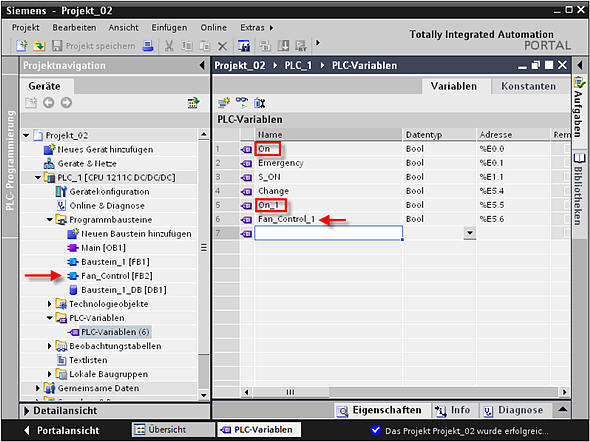
\includegraphics[width=0.8\linewidth]{images/Variablentabelle.jpg}
	\caption{Übersicht der Variablentabelle in TIA Portal \cite{siemens_vars2024}}
	\label{fig:uebersicht_tia}
\end{figure}

Das Hauptprogramm besteht aus sogenannten \textbf{POUs} (Program Organization Units, deutsch: Programmorganisationseinheiten).  
Diese werden in drei Arten unterteilt: \textbf{Programme}, \textbf{Funktionen (FC)} und \textbf{Funktionsbausteine (FB)}.  
Die Realisierung dieser POUs in \textit{Siemens TIA Portal} wurde bereits im vorherigen Kapitel (vgl. \ref{label}) beschrieben.  
Nachfolgend wird die Bedeutung und Funktion der einzelnen Organisationseinheiten erläutert.

Das \textbf{Programm} dient der Realisierung komplexer Abläufe, beispielsweise von Schrittketten oder Hauptlogiken.  
Eine \textbf{Funktion (FC)} ist mit einer C-ähnlichen Funktion vergleichbar. Sie verarbeitet eine oder mehrere Eingangsvariablen und gibt nach der Abarbeitung ein Ergebnis zurück.  
Gemäß IEC 61131-3 können Funktionen jedoch nicht rekursiv aufgerufen werden und besitzen kein eigenes Speicherverhalten, d.\,h. sie können keine Werte dauerhaft speichern \cite{Seitz.2021}.  
Ein einfaches Beispiel hierfür ist ein logisches \textbf{UND-Gatter}.

Ein \textbf{Funktionsbaustein (FB)} hingegen besitzt ein internes Gedächtnis und kann Werte über mehrere Zyklen hinweg speichern. Dadurch eignet er sich besonders für Zustandsautomaten oder speichernde Operationen.  
Ein klassisches Beispiel hierfür ist ein \textbf{RS-Flip-Flop}.

Für die Programmierung stehen verschiedene Sprachen nach IEC 61131-3 \cite{IEC6113-3_2022} zur Verfügung:
\begin{itemize}
	\item KOP (Kontaktplan),
	\item AWL (Anweisungsliste),
	\item FUP/FBS (Funktionsplan / Funktionsbausteinsprache),
	\item ST/SCL (Structured Text / Structured Control Language)\footnote{SCL ist die Siemens-spezifische Implementierung der nach IEC~61131-3 genormten Programmiersprache Structured Text (ST) im TIA Portal \cite{Kanngießer}.}
\end{itemize}

In modernen Industrieanlagen werden überwiegend \textbf{FUP} und \textbf{ST} eingesetzt. Diese Programmiersprachen zeichnen sich durch eine gute Übersichtlichkeit und eine effiziente Fehleranalyse aus.  
Trotzdem bestehen zwischen beiden Varianten wesentliche Unterschiede, die in Tabelle~\ref{tab:vergleich_fup_st} dargestellt sind.

\begin{table}[H]
	\centering
	\begin{tabular}{|p{7cm}|p{7cm}|}
		\hline
		\textbf{ST / SCL (Structured Text / Structured Control Language)} & \textbf{FUP (Funktionsplan)}\\
		\hline
		Textbasierte Programmiersprache & Grafische Programmiersprache\\
		\hline
		Hochsprachenähnlich (z.\,B. C, Pascal) & Verwendung grafischer Symbole und logischer Verknüpfungen\\
		\hline
		Klare und kompakte Struktur & Gefahr der Unübersichtlichkeit bei komplexen Programmen\\
		\hline
		Besonders geeignet für mathematische und logische Operationen & Gut geeignet für einfache logische Abläufe\\
		\hline
	\end{tabular}
	\caption{Vergleich zwischen ST (Structured Text) und FUP (Funktionsplan) \cite{siemens_programmieren}}
	\label{tab:vergleich_fup_st}
\end{table}

Wie aus der Tabelle hervorgeht, bietet die textbasierte Programmiersprache \textbf{ST} insbesondere bei komplexen Strukturen und mathematischen Berechnungen erhebliche Vorteile.  
\textbf{FUP} hingegen ist für Einsteiger leichter verständlich und eignet sich für überschaubare Steuerungslogiken.  
Mit zunehmender Komplexität der Abläufe stößt FUP jedoch schnell an seine Grenzen, da die grafische Darstellung umfangreicher Strukturen unübersichtlich werden kann \cite{siemens_programmieren}.  
Um die genauen Unterschiede zu erläutern, sollen zunächst grundlegende Elemente der einzelnen Sprachen eingeführt werden.  
Zunächst erfolgt eine Beschreibung der wichtigsten Grundbausteine in FUP.

\subsubsection*{Wichtige Grundfunktionen (UND, ODER, NICHT) in FUP}
\begin{figure}[H]
	\centering
	\begin{subfigure}[b]{0.49\textwidth}
		\centering
		\includegraphics[width=0.8\linewidth]{images/UND_GATTER}
		\caption{\textbf{UND\_Gatter} \cite{Hering}}
	\end{subfigure}
	\hfill
	\begin{subfigure}[b]{0.49\textwidth}
		\centering
		\includegraphics[width=0.8\linewidth]{images/ODER_GATTER}
		\caption{\textbf{ODER\_Gatter} \cite{Hering}}
	\end{subfigure}
	
	\vspace{1cm}
	
	\begin{subfigure}[b]{0.49\textwidth}
		\centering
		\includegraphics[width=0.8\linewidth]{images/NOT_GATTER}
		\caption{\textbf{NOT\_Gatter} \cite{Hering}}
	\end{subfigure}
	\caption{Darstellung der logischen Grundfunktionen in FUP}
	\label{fig:grundfunktionen_fup}
\end{figure}

\subsubsection*{Wichtige Funktionsbausteine in FUP}
\begin{figure}[H]
	\centering
	\begin{subfigure}[b]{0.49\textwidth}
		\centering
		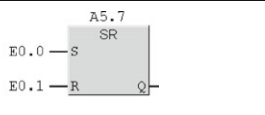
\includegraphics[width=0.8\linewidth]{images/SR_FLIPFLOP}
		\caption{\textbf{SR\_FLIPFLOP} \cite{Hering}}
	\end{subfigure}
	\hfill
	\begin{subfigure}[b]{0.49\textwidth}
		\centering
		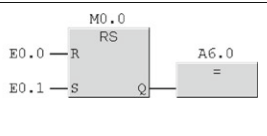
\includegraphics[width=0.8\linewidth]{images/RS_FLIPFLOP}
		\caption{\textbf{RS\_FLIPFLOP} \cite{Hering}}
	\end{subfigure}
	
	\vspace{1cm}
	
	\begin{subfigure}[b]{0.49\textwidth}
		\centering
		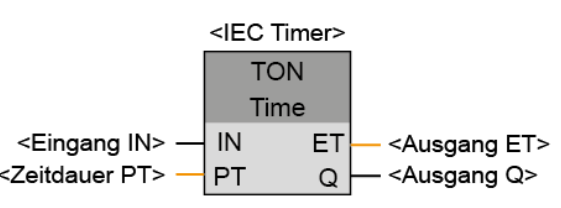
\includegraphics[width=0.8\linewidth]{images/TON}
		\caption{\textbf{Einschaltverzögerung (TON)} \cite{Hering}}
	\end{subfigure}
	\hfill
	\begin{subfigure}[b]{0.49\textwidth}
		\centering
		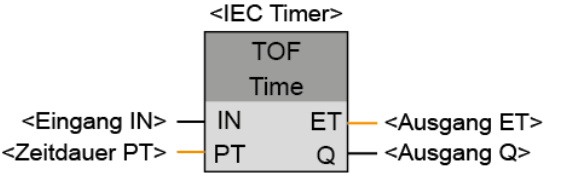
\includegraphics[width=0.8\linewidth]{images/TOF}
		\caption{\textbf{Ausschaltverzögerung (TOF)} \cite{Hering}}
	\end{subfigure}
	\caption{Darstellung wichtiger Funktionsbausteine in FUP}
	\label{fig:funktionsbausteine_fup}
\end{figure}

In den obigen Abbildungen sind die wichtigsten Grundfunktionen und Funktionsbausteine in \textbf{FUP} dargestellt.  
Mit diesen können diverse Abläufe realisiert werden, wie beispielsweise einfache Förderbandsteuerungen.  
Komplexe, lange Abläufe sind jedoch sehr aufwendig zu realisieren. Für eine SPS ist es daher gebräuchlich, hierfür auf \textbf{ST/SCL} auszuweichen.  
In FUP können ebenfalls mathematische Operationen durchgeführt werden. Für Berechnungen existieren spezielle Bausteine. Allerdings ist es schwierig, längere Rechenvorgänge übersichtlich darzustellen, da die Struktur schnell unübersichtlich wird.  
Aus diesem Grund werden für sämtliche mathematische Operationen häufig Berechnungen in \textbf{ST/SCL} durchgeführt.  
Beim vorliegenden Modell, dem Hochregallager, wurde beispielsweise die Positionsermittlung der Lagerplätze für das automatisierte Einlagern im vergangenen Studienprojekt in \textbf{SCL} realisiert.
\subsubsection*{Grundlegende Anweisungen in SCL}
Im vorliegenden Projekt wird mit einer Siemens SPS gearbeitet. Somit ist SCL (Structured Control Language) der Standard im Bereich textbasierte Programmierung.\\
Hierbei gibt es einige konkrete Anweisungen, welche eine übersichtliche Programmierung gewährleisten.\\
Zu diesen zählen:
\begin{itemize}
	\item \textbf{Zuweisungen:} \texttt{Variable := Wert;}  
	Beispiel: \texttt{Motor\_Start := TRUE;}
	\item \textbf{Bedingte Anweisungen (IF-Strukturen):}  
	\texttt{IF Sensor = TRUE THEN Motor := TRUE; END\_IF;}
	\item \textbf{Mehrzweigige Bedingungen (IF-ELSIF-ELSE):}  
	\texttt{IF Temp > 50 THEN Alarm := TRUE; ELSIF Temp > 30 THEN Warning := TRUE; ELSE Alarm := FALSE; END\_IF;}
	\item \textbf{Schleifenstrukturen:}  
	\texttt{FOR i := 1 TO 5 DO Count := Count + 1; END\_FOR;}
	\item \textbf{Vergleiche und logische Operatoren:}  
	\texttt{AND, OR, NOT, >, <, =, >=, <=}
\end{itemize}
Diese Anweisungen ermöglichen selbst komplexe Programme zu realisieren. Es können mathematische Berechnungen deutlich einfacher durchgeführt werden als beispielsweise in der Programmiersprache \textbf{FUP}.
\subsubsection*{Vergleich SCL - FUP}
Die Programmiersprachen \textbf{FUP} und \textbf{SCL} werden beide für die Programmierung speicherprogrammierbarer Steuerungen verwendet.\\
Da \textbf{SCL} eine Siemens-eigene Sprache ist, konzentriert sich dieser Vergleich ausschließlich auf \textbf{STEP 7}.\\
Wie bereits erwähnt, ermöglicht \textbf{FUP} eine einfache blockbasierte Programmierung.\\
\textbf{FUP} eignet sich besonders für einfache Anwendungen, wie beispielsweise die Ansteuerung von Drehstrommotoren. Auch für einfache Schrittketten ist \textbf{FUP} gut geeignet.\\
Mit zunehmender Programmkomplexität leidet jedoch die Übersichtlichkeit, was zu einer erhöhten Fehleranfälligkeit führen kann.\\
Um diese Probleme zu vermeiden, wird in großen Produktionsanlagen mit komplexen Abläufen überwiegend textbasiert, also in \textbf{SCL}, programmiert.
\newpage
Die folgenden Darstellungen vergleichen beide Sprachen und verdeutlichen ihre Unterschiede.\\
Dargestellt ist eine einfache Förderbandsteuerung in \textbf{FUP} und \textbf{SCL} im TIA Portal.
\begin{figure}[H]
	\centering
	\label{fig: Beispiel FUP}
	\begin{subfigure}[b]{0.49\textwidth}
		\centering
		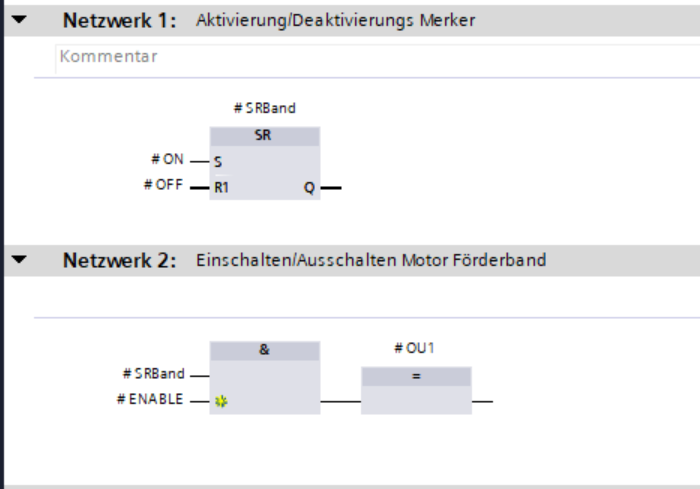
\includegraphics[width=0.8\linewidth]{images/PrgBeispiel_FUP}
		\caption{Funktionsbaustein zur Steuerung des Förderbands}
	\end{subfigure}
	\hfill
	\begin{subfigure}[b]{0.49\textwidth}
		\centering
		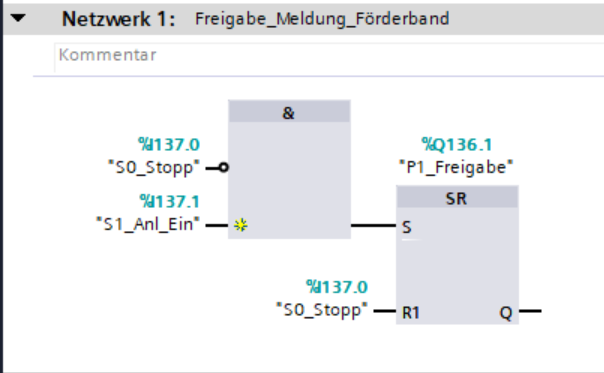
\includegraphics[width=0.8\linewidth]{images/PrgBeispiel_FUP_2}
		\caption{Freigabe im Haupt-OB}
	\end{subfigure}
	
	\vspace{0.5cm}
	
	\begin{subfigure}[b]{0.45\textwidth}
		\centering
		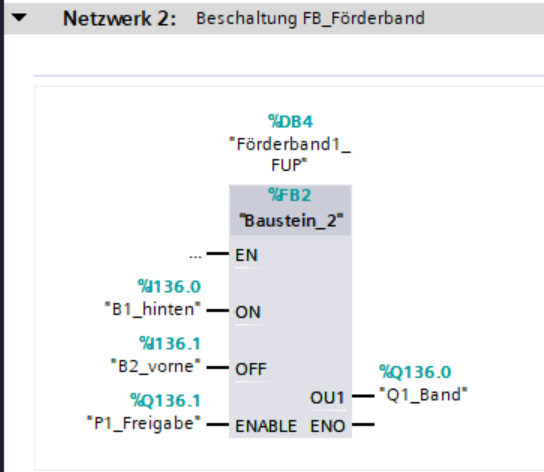
\includegraphics[width=0.8\linewidth]{images/PrgBeispiel_FUP_3}
		\caption{Einbindung des FBs im Haupt-OB}
	\end{subfigure}
	\caption{Realisierung der Förderbandsteuerung in \textbf{FUP}}
\end{figure}

\begin{figure}[H]
	\centering
	% Erste Spalte – Förderband-Baustein
	\begin{subfigure}[t]{0.4\textwidth}
		\centering
		\begin{lstlisting}[language=Pascal]
IF #OFF THEN
	#SR_Band := FALSE;	
ELSIF #ON THEN
	#SR_Band := TRUE;
END_IF;
			
#OU1 := #SR_Band AND #ENABLE;
		\end{lstlisting}
		\caption{SCL-Code des Förderband-Bausteins}
		\label{lst:Foerderband}
	\end{subfigure}
	\hfill
	% Zweite Spalte – Aufruf im Hauptprogramm
	\begin{subfigure}[t]{0.4\textwidth}
		\centering
		\begin{lstlisting}[language=Pascal]
IF NOT "S0_Stop" AND "S1_Anl_Ein" THEN
	"Pl_Freigabe" := TRUE;
ELSIF "S0_Stop" THEN
	"Pl_Freigabe" := FALSE;
END_IF;
			
"Foerderband"(
OFF    := "B2_vorne",
ON     := "B1_hinten",
ENABLE := "Pl_Freigabe",
OU1    => "Q1_Band");
		\end{lstlisting}
		\caption{Aufruf des Förderband-Bausteins im Hauptprogramm}
		\label{lst:Foerderband_call}
	\end{subfigure}
	\caption{Realisierung des Förderbandprogramms in \textbf{SCL}}
	\label{fig:Foerderband_Listing}
\end{figure}

Anhand des Beispiels wird deutlich, dass \textbf{FUP} auf den ersten Blick leichter verständlich wirkt, da es sich um die grafische Verschaltung logischer Funktionen handelt.\\
Auf den zweiten Blick zeigt sich jedoch, dass der Programmieraufwand deutlich höher ist als in \textbf{SCL}. In \textbf{SCL} kann dieselbe Funktionalität mit wenigen, klar strukturierten Codezeilen realisiert werden, ohne das Programm mit zusätzlichen Netzwerken zu überladen.\\
Zusammenfassend lässt sich festhalten, dass sowohl \textbf{FUP} als auch \textbf{SCL} ihre jeweiligen Vor- und Nachteile besitzen. Je nach Anwendung und Komplexität des Prozesses fällt die Entscheidung für die eine oder die andere Programmiersprache.





\newpage
\printbibliography
\end{document}